\documentclass{article}
\usepackage{graphicx} % Required for inserting images
\usepackage{graphicx} % Required for inserting images
% Change page dimensions
\usepackage[margin=1in]{geometry}
\usepackage{amsmath}
\usepackage{amssymb}
\usepackage{subcaption} % in preamble
\usepackage{algorithm}
\usepackage{algpseudocode}
\usepackage{minted}
\usemintedstyle{friendly} % or bw, colorful, etc.
\usepackage{datetime}
\usepackage{booktabs} % For better-looking tables
\usepackage{array}    % For additional column formatting
\usepackage{threeparttable}
\usepackage{tabularx}
\usepackage{subcaption} % Add to preamble


\title{AMIC Uncertainty – Bayesian Variational}
\author{Leon King}
\date{\today} % This will insert current date
% introduce paper.bib
\usepackage[utf8]{inputenc}

% Bibliography setup
\usepackage[backend=biber, style=numeric, sorting=none]{biblatex}
\addbibresource{paper.bib} % Replace with your .bib filename

% Load hyperref LAST in your preamble
\usepackage{hyperref}

% Optional: Configure the appearance of the hyperlinks
\hypersetup{
    colorlinks=true,       % Colours the text instead of drawing a box
    linkcolor=blue,        % Colour for internal links (e.g., TOC, equations)
    citecolor=red,         % Colour for bibliographic citations
    urlcolor=magenta       % Colour for URL links
}

\begin{document}

\maketitle

\section{Introduction}
AMIC is a natural language \textbf{shallow} neural network model that integrates layers of self-attention with logistic linear regression methods to calculate sentiment scores at the word and document level. This AMIC model performs well on a wine review dataset with approximately 89\% accuracy in the test set. However, the current architecture of the AMIC model can only generate point estimations in either continuous regression or classification tasks. As a data scientist and statistician, I always want to know the level of uncertainty about the estimation of points. This is why we would like to modify the AMIC to produce uncertainty for prediction point estimations.

\subsection{introduce AMIC}
In this subsection, I will introduce the basic architecture of the original AMIC model as shown in the figure \ref{fig:amic}. The AMIC model has two layers of nested regressions inside. The out-of-context word embeddings $x_{ij}$ from the outer source are first trained to have contextual word embeddings $a_{ij}^P$ with the transformer-styled self-attention layer. The first layer in the blue box is to select the sentiment word denoted by $\delta_{ij}$ in the document with the logistic regression, given the input contextual word embeddings $a_{ij}^P$. The math formula for this layer is $$\begin{aligned}
u_{i j} & =a_{i j}^P b, \\
\delta_{i j} & =\frac{1}{1+e^{-u_{i j}}}
\end{aligned}$$ where the $b$ is the logistic coefficients. The second layer in the red box is to produce the sentiment score $Z_{ij}$ for each word and get the document-level sentiment $Z_i$ with another logistic regression. The math formula for this layer is $$\begin{aligned}
& Z_{i j}=\delta_{i j} a_{i j}^L \beta, \\
& Z_i=\frac{\sum_{j=1}^m Z_{i j}}{m}, \\
& \hat{y}_i=\mathbf{1}_{[0.5,1]}\left(\operatorname{sig}\left(Z_i\right)\right)
\end{aligned}$$ where $\beta$ is the layer two logistic regression coefficient, $a_{ij}^L$ is the contextual word embeddings trained with another self-attention layer, $m$ is the total number of words in a document, $sig$ is the sigmoid function, $\hat{y_i}$ is the predicted the document sentiment label. This model also has three penalty terms: $p_{i1}, p_{i2}, p_{i3}$. $p_{i1}$ encourages peak-ness sentiment word selection. $p_{i2}$ encourages the sparsity of sentiment words. $p_{is}$ stabilizes the sentiment scores $Z_{ij}$.

\begin{figure}
    \centering
    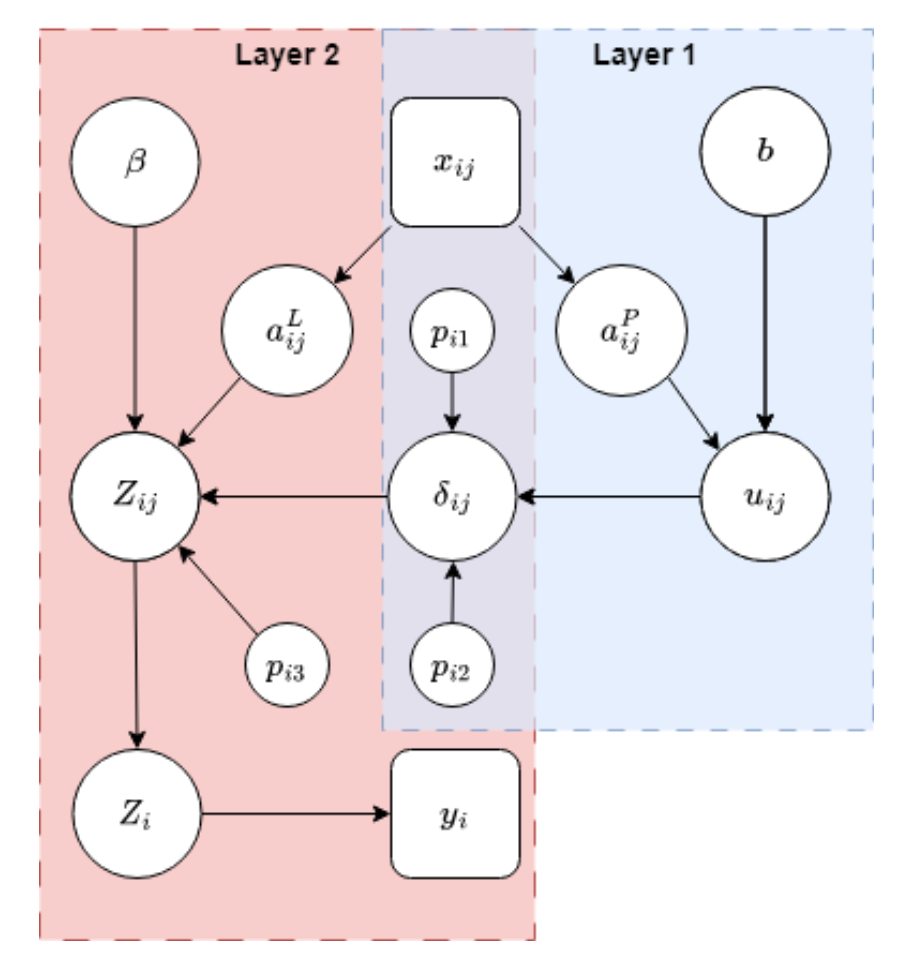
\includegraphics[width=0.5\linewidth]{amic.png}
    \caption{Model Structure of AMIC}
    \label{fig:amic}
\end{figure}
Now I introduce the basic implementation part in the AMIC model. We used the PyTorch platform to write the code. We have four essential classes, \textit{SelfAttention}, \textit{Mask\_block}, \textit{Sentiment\_block}, \textit{Synthesizer}. The blue box layer one is implemented in the \textit{Mask\_block}, and the logistic regression part of layer two is implemented in \textit{Sentiment\_block}. The final document-level prediction is implemented into the \textit{Synthesizer}. Both \textit{Mask\_block} and \textit{Sentiment\_block} contain a \textit{SelfAttention} layer to train the contextual self-attention word-level embeddings, $a_{ij}^P, a_{ij}^L$. 

\subsection{Interface between AMIC and new Bayesian Variational}
In this section, we discuss how the AMIC model transitions into the new Bayesian variational layer. The interface happens at layer two. Layer two has one primary output, $a_{ij}^L$, which is used in the Bayesian layer, representing the contextual word-level embeddings. The other output that is used in the Bayesian layer is the padding mask vector from the \textit{Mask\_block}. Next, we used the word-level embeddings $a_{ij}^L$ and padding mask $p_i$ to compute the pooled document-level embeddings $h_i$ for the Bayesian layer. The following formula outlines the calculation of this pooled document-level embedding in three steps. The first step is to use the padding mask vector $p_{i}$ to zero out all padding tokens: $$p_{ij} \times a_{ij}^L$$ The second step is to sum this result over the token axis $j$: $$\sum_{j=1}^T (p_{ij} \times a_{ij}^L)$$ The third step is to divide this by number of valid tokens: $$h_i=\frac{\sum_{j=1}^T (p_{ij} \times a_{ij}^L)}{Max(1,\sum_j p_{ij})}$$ where $i$ means the index of document and $j$ means the index of word in the document $i$. However, there are several different methods for computing the pooled document-level embeddings. This is one of them, and we can keep trying other ways. We pass this document-level embedding $h_i$ into a dropout layer, then into our new Bayesian Variational Layer to calculate the uncertainty and the final loss function. 

I drew a flow diagram that is similar to Figure 1 AMIC \ref{fig:amic} to display the high-level model structure of this Bayesian Variational AMIC model \ref{fig:bamic}.
\begin{figure}[!ht]
    \centering
    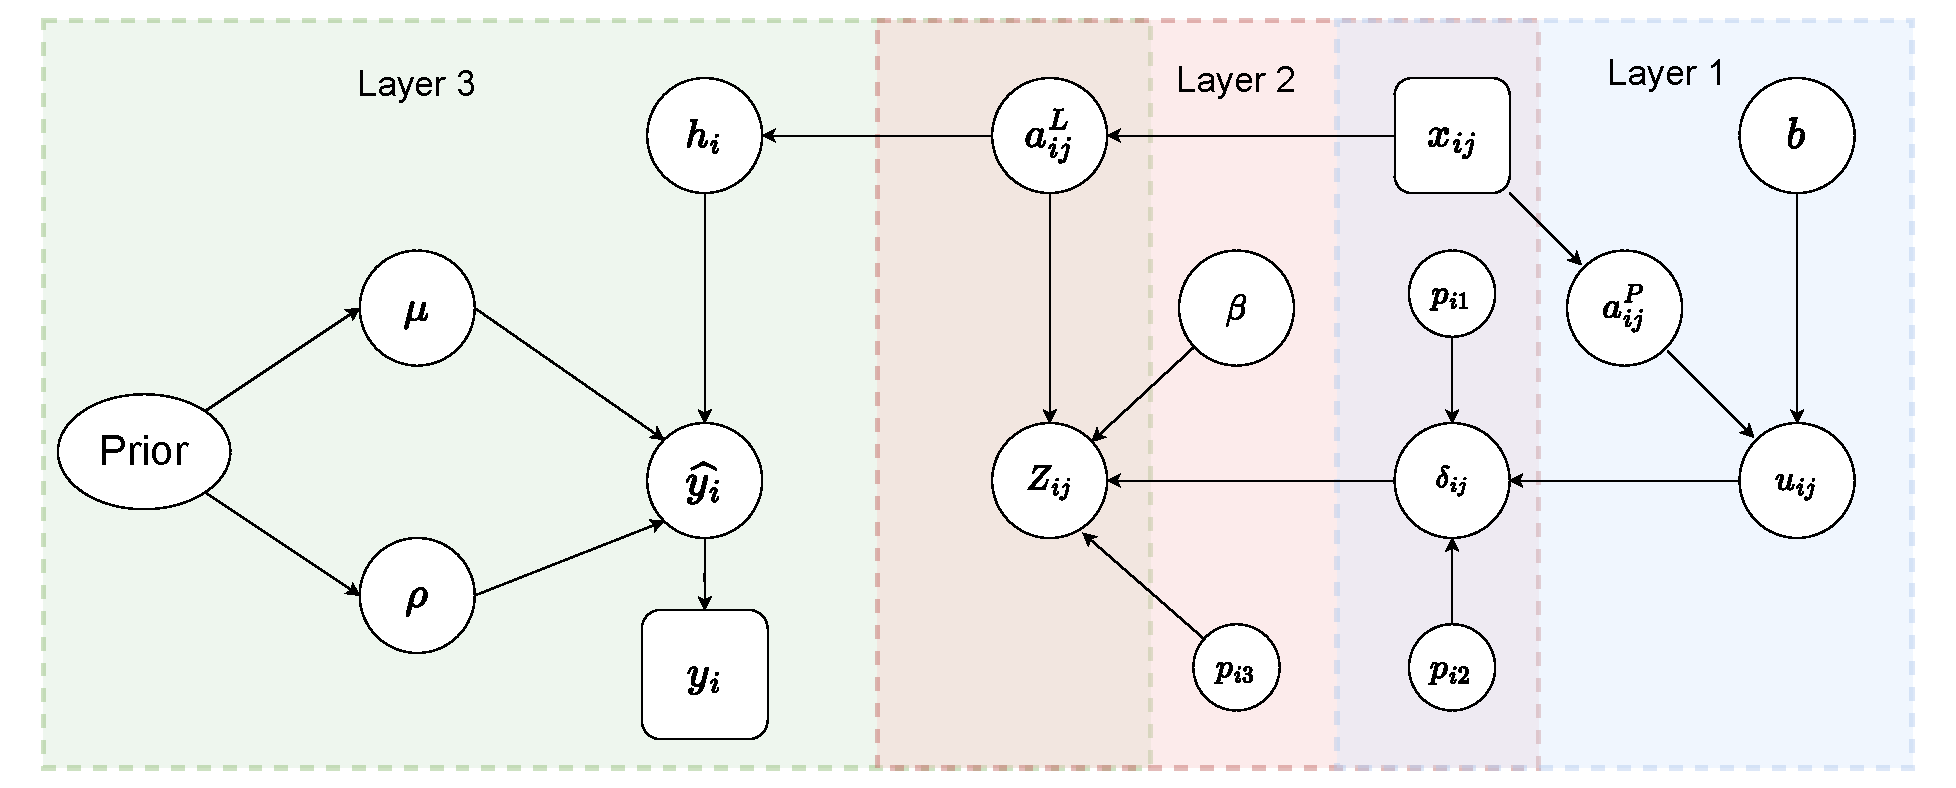
\includegraphics[width=1\linewidth]{BAMIC.pdf}
    \caption{Model Structure of BAMIC}
    \label{fig:bamic}
\end{figure}
The first blue box layer and the second red box layer are identical to the original AMIC model. The new Bayesian layer is the third green box layer. The contextual word embeddings $a_{ij}^L$ are the input to Layer 3. Then, all $a_{ij}^L$ values from one document are pooled to produce the document-level embedding $h_i$. $h_i$ is sent into the Bayesian Variational layer to produce the final prediction $\hat{y}_i$ of document i that is used to compute the final loss function. During the training, posterior parameters $\mu$ and $\rho$ are trained to give weights of this Bayesian layer given the prior input. This is a simplified illustration of Bayesian AMIC; the more detailed low-level diagram is shown in Figure \ref{fig:Bayes}.    


\section{Methods}
There are two major methods to produce uncertainty for a neural network model. One method is simple and quick, but less accurate. The method is to add a dropout layer to the AMIC model, then repeat the forward pass of the model to generate a sample of predictions. Finally, the mean, variance, lower quantile, upper quantile and any other statistics can be calculated from these Monte Carlo samples. The second method is a more complicated but more accurate method for calculating uncertainty based on the \textbf{Variational Bayesian} approach. The method is to add one or more Bayesian layers to the model. In the following sections, we will discuss more details and the architecture of this method for the AMIC model. 

\section{Bayesian Variational Method}
The core principle of this method is to learn the probability distributions of weights and biases of neural networks. The following graphs \ref{fig:bayes} from the paper 'Weight Uncertainty in Neural Networks' published by Google DeepMind in 2015 \textcite{blundell2015weightuncertaintyneuralnetworks} illustrate this core principle.
\begin{figure}[!ht]
    \centering
    \includegraphics[width=0.5\linewidth]{bayes.png}
    \caption{The left network has only point weights and biases, while the right network has probability distributions}
    \label{fig:bayes}
\end{figure}
The left network is a traditional neural network with point learned weights. The right network is the Bayesian Variational with probability weight distribution. Every weight distribution has a different distribution. Passing through the forward function many times generates a sample of weights. So do the final predictions. Generally speaking, the exact posterior distributions of weights in a neural network are intractable due to the large number of parameters, and there does not exist an analytical formula for a neural network. This is why the paper authors proposed a variational approximation to the Bayesian posterior. If the data used to train this Bayes model is small, the uncertainty of outcomes can be large. However, as the data increases, the uncertainty of outcomes from this Bayesian neural network can decrease as more data is collected to better understand the environment.    

\section{Mathematics behind the Bayesian Variational NN}
The core principle of this method is to find a tractable posterior distribution to approximate the intractable posterior distribution. If the tractable distribution of weights is $q(w|\theta)$, then we need to minimize the Kullback-Leibler (KL) divergence between the true Bayesian posterior $P(w|D)$ and the approximated distribution, $q(w|\theta)$. 
$$\begin{aligned}
\theta^{\star} & =\arg \min _\theta \mathrm{KL}[q(\mathbf{w} \mid \theta) \| P(\mathbf{w} \mid \mathcal{D})] \\
& =\arg \min _\theta \int q(\mathbf{w} \mid \theta) \log \frac{q(\mathbf{w} \mid \theta)}{P(\mathbf{w}) P(\mathcal{D} \mid \mathbf{w})} \mathrm{d} \mathbf{w} \\
& =\arg \min _\theta \mathrm{KL}[q(\mathbf{w} \mid \theta) \| P(\mathbf{w})]-\mathbb{E}_{q(\mathbf{w} \mid \theta)}[\log P(\mathcal{D} \mid \mathbf{w})]
\end{aligned}$$ This derivation is from the Google DeepMind paper by \textcite{blundell2015weightuncertaintyneuralnetworks} I introduced before. Then they also get the costing function for this setup as follows: 
$$\mathcal{F}(\mathcal{D}, \theta)=\mathrm{KL}[q(\mathbf{w} \mid \theta) \| P(\mathbf{w})]  -\mathbb{E}_{q(\mathbf{w} \mid \theta)}[\log P(\mathcal{D} \mid \mathbf{w})]$$ where $P(\mathbf{w})$ is prior distribution for weights $\mathbf{w}$, $P(D|\mathbf{w})$ is the data likelihood function given the current weights. During the training, the data-dependent part $\mathbb{E}_{q(\mathbf{w} \mid \theta)}[\log P(\mathcal{D} \mid \mathbf{w})]$ of this cost function is going to make the weights as large as it can be to maximize the data likelihood function and explain the data variance as it were in a traditional neural network training. However, on the other side, the KL divergence part $\mathrm{KL}[q(\mathbf{w} \mid \theta) \| P(\mathbf{w})]$ is going to simplify the weight distribution closer to the simple prior distribution of weights as a regularization term. The best training result is to find the trade-off sweet spot between two extremes. 

However, if we select some complicated prior and variational posterior distributions, it's impractical to compute the closed form of this cost function $\mathcal{F}(\mathcal{D}, \theta)$. Thus, under certain conditions, the unbiased Monte Carlo estimations were proposed to represent the cost function in the training process. 
$$\mathcal{F}(\mathcal{D}, \theta) \approx \frac{1}{n}\sum_{i=1}^n \left(\log q\left(\mathbf{w}^{(i)} \mid \theta\right)- \log P\left(\mathbf{w}^{(i)}\right) -\log P\left(\mathcal{D} \mid \mathbf{w}^{(i)}\right)\right)$$ where $\mathbf{w}^{i}$ is $i-th$ Monte Carlo sample from the variational posterior $q(\mathbf{w^{(i)}}|\theta)$.

\section{Deploy this cost function into AMIC model}
The goal of AMIC model is to predict the classification of binary labels. We need to modify the cost function mentioned above to better suit our supervised text sentiment analysis. In our dataset, for example, the wine review data has the ground truth labels. We changed the data-dependent part $-\mathbb{E}_{q(\mathbf{w} \mid \theta)}[\log P(\mathcal{D} \mid \mathbf{w})]$ into the traditional binary cross-entropy loss function between logits and true labels, call \textbf{NLL}. We set up the prior and variational posterior distributions as a Gaussian distribution to simplify our derivations, and it's usually the golden standard to start with a normal distribution in any Bayesian inference. We also added two penalty terms, $p_1$ and $p_3$, into our loss function to regularize the training. The first penalty term is the sparsity term $p_1$, which encourages fewer tokens to be important: $$p_{1b}=\sum_{t=1}^Tm_{b,t}$$ where $m_{bt}$ is a word-level importance indication score.  The second penalty term is the peak-ness term, which encourages the token's important scores to be either 0 or 1, $$p_{3b}=\sum^T_{t=1}(m_{bt}(1-m_{bt}))^2.$$ When $m_{bt}$ is 0.5, $p_3$ reaches the maximum value, where $m_{bt}$ is a word-level important indication score. 

The final cost function for our Bayesian AMIC model is as follows:
\begin{equation}
    \textbf{Loss}(D, \mu, \rho) = \textbf{cross-entropy}(logits(D), y)+\beta \cdot \textbf{KL}(q(w(\mu,\rho),\theta)||P(w))+\lambda_1 \cdot E(p_1)+\lambda_3 \cdot E(\sqrt{p_3 + \epsilon})
    \label{eq:loss}
\end{equation} where logits are the final layer outcome in the neural network, $y$ is true labels, $\beta$ is the degree of how much we want KL divergence to regularize the cost function: the bigger $\beta$ is, the more the model would push the variational posterior to the prior, $\lambda_1$ is the degree of how much sparsity penalty to regularize the cost function, and $\lambda_3$ is the degree of how much peakness penalty to regularize the cost function, $\epsilon$ is a tiny positive number $10^{-8}$ to make sure the square root a positive number, $E$ is the expectation. $D$ is the dataset, $\theta = (\mu, \rho)$ is the Gaussian distribution parameter we would train and update in our Bayesian variational AMIC model. Throughout neural network training, the fundamental raw parameters are usually spread across all real numbers; however, the standard deviation of a normal distribution is positive. Thus, we use the transformation from proposed by \cite{blundell2015weightuncertaintyneuralnetworks} $\rho$ to $\sigma$ as follows: $$\sigma=\log (1+\exp (\rho)) \in (0,+\infty),\; \rho\in (-\infty,+\infty)$$

Next, we define the KL divergence function for the prior and variational posterior distribution as follows: $$\mathrm{KL}(q \| p)=\int q(x) \log \frac{q(x)}{p(x)} d x=\mathbb{E}_{x \sim q}[\log q(x)-\log p(x)]$$ By the definition, the KL divergence is non-negative and asymmetric. In our Bayesian linear layer, we set up the prior weights to be simple normal distribution $p(w)\sim N(0, \sigma^2_p)$ for each weight and bias independently. We selected the variational posterior normal for weights and biases as it were conjugate in most basic Bayesian inference $q(w)=N(\mu, \sigma^2)$. 

When the prior and approximated distributions are all normal, the KL divergence has a closed form. The $\log q(w,\theta)$ is the following:
$$\log q(w)=-\frac{1}{2}\left[\log \left(2 \pi \sigma^2\right)+\frac{(w-\mu)^2}{\sigma^2}\right]$$ The prior $\log p(w)$ is the following: $$\log p(w)=-\frac{1}{2}\left[\log \left(2 \pi \sigma_p^2\right)+\frac{w^2}{\sigma_p^2}\right]$$ Then we take expectations for both logs. The random variable is weight $w$. The first expectation would be $$\mathbb{E}_q\left[(w-\mu)^2\right]=\sigma^2$$ the variance of weights. The second expectation would be $$\mathbb{E}_q\left[w^2\right]=\sigma^2+\mu^2$$ Lastly, we plug these two expectations into the KL divergence, we have the following: $$\begin{aligned}
\mathrm{KL}(q \| p) & =-\frac{1}{2} \log \left(2 \pi \sigma^2\right)+\frac{1}{2} \log \left(2 \pi \sigma_p^2\right)-\frac{1}{2} \cdot 1+\frac{1}{2} \frac{\sigma^2+\mu^2}{\sigma_p^2} =\log \frac{\sigma_p}{\sigma}+\frac{\sigma^2+\mu^2}{2 \sigma_p^2}-\frac{1}{2} .
\end{aligned}$$ The above is the KL divergence for one single weight. We need to sum up all weights' and biases' KL divergence by independent assumption as follows: 
\begin{equation}
    \mathrm{KL}_{\text {Bayesian Layer}}=\sum_{i \in W}\left(\log \frac{\sigma_p}{\sigma_i}+\frac{\sigma_i^2+\mu_i^2}{2 \sigma_p^2}-\frac{1}{2}\right)+\sum_{j \in b}\left(\log \frac{\sigma_p}{\sigma_j}+\frac{\sigma_j^2+\mu_j^2}{2 \sigma_p^2}-\frac{1}{2}\right)
    \label{eq:KL}
\end{equation}

\section{Bayesian AMIC model architecture}
\subsection{Bayesian Linear Layer}
The idea of combining the Bayesian variational method with the original AMIC is to add one more Bayesian layer to the AMIC model. However, the input to this new Bayesian layer is a pooled review-level embedding from the sentiment block and mask block of the original AMIC model. The sentiment block produces contextual word-level embeddings for each review, $F_b$, dimension 300 by 1. The mask block produces the padding masks for each review, $m_b$. Thus, the pooled review-level embedding is calculated as follows: $$h_b = \frac{m_b^T \cdot F_b}{1^T\cdot m_b + \epsilon}$$ Once we have these attention-based contextual token features, we pass them through a dropout layer and then pass them into the Bayesian layer. This Bayesian layer is implemented by \textbf{BayesLinear(nn.Module)}. The first step for this layer is to initialize the training parameters $\mu$ and $\rho$ for weights and biases, and specify a prior sigma. Then we define two \textbf{F.softplus} functions to transform $\rho$ to $\sigma$ by $\sigma=\log (1+\exp (\rho))$. Next, we define a function to calculate the KL divergence for all weights and biases, returning a single scale number according to the formula in equation \ref{eq:KL}. The last step is to define the forward pass function to construct the weights and biases by training parameters $\mu$, $\rho$, and random standard normal values $\epsilon$ by $\mathbf{w}=\mu+\log (1+\exp (\rho)) \circ \epsilon$, where $\epsilon \sim \mathcal{N}(0, I)$. We can repeat sampling $\epsilon \sim \mathcal{N}(0, I)$ as many times as we want to form a sample of neural networks to produce different logits and probabilities. This procedure gives us a posterior sampling distribution to make any Bayesian inference of interest. This forward pass function returns a fully connected linear layer \textbf{logit} given the input $h_b$ by the above-constructed weights and biases without managing the weights and biases as parameters within an \textbf{nn.Module}. The following code \ref{lst:bayes} is the \textbf{BayesLinear(nn.Module)}.
\begin{listing}[!ht]
\caption{The Python Class for BayesLinear(nn.Module)}
\label{lst:bayes}
\begin{minted}[fontsize=\small, breaklines, linenos]{python}
class BayesLinear(nn.Module):
    """Factorized Gaussian posterior; prior N(0, sigma_p^2 I)."""
    def __init__(self, in_features, out_features, prior_sigma=1.0, init_rho=-3.0):
        super().__init__()
        self.weight_mu  = nn.Parameter(torch.zeros(out_features, in_features))
        self.weight_rho = nn.Parameter(torch.full((out_features, in_features), float(init_rho)))
        self.bias_mu    = nn.Parameter(torch.zeros(out_features))
        self.bias_rho   = nn.Parameter(torch.full((out_features,), float(init_rho)))
        self.register_buffer("prior_sigma", torch.tensor(float(prior_sigma)))

    @property
    def weight_sigma(self):
        return F.softplus(self.weight_rho) + 1e-8

    @property
    def bias_sigma(self):
        return F.softplus(self.bias_rho) + 1e-8

    def kl(self) -> torch.Tensor:
        w_mu, w_sigma = self.weight_mu, self.weight_sigma
        b_mu, b_sigma = self.bias_mu,   self.bias_sigma
        p_sigma = self.prior_sigma
        kl_w = torch.log(p_sigma / w_sigma) + (w_sigma**2 + w_mu**2) / (2 * p_sigma**2) - 0.5
        kl_b = torch.log(p_sigma / b_sigma) + (b_sigma**2 + b_mu**2) / (2 * p_sigma**2) - 0.5
        return kl_w.sum() + kl_b.sum()

    def forward(self, x, sample: bool = True):
        if self.training or sample:
            W = self.weight_mu + self.weight_sigma * torch.randn_like(self.weight_mu)
            b = self.bias_mu   + self.bias_sigma   * torch.randn_like(self.bias_mu)
        else:
            W, b = self.weight_mu, self.bias_mu
        return F.linear(x, W, b)
\end{minted}
\end{listing}

\subsection{Synthesizer Layer}
After we have the logit output from the previous Bayesian Linear Layer, we define a new class called \textbf{SynthesizerVIvec(nn.Module)} to calculate logits and probabilities. The pooled review-level embeddings first pass through a dropout layer, and then pass through the previously defined \textbf{BayesLinear(nn.Module)} layer to produce single-scale logits. The last step is to apply the \textbf{sigmoid} function $\sigma(x)=\frac{1}{1+e^{-x}}$ to the logits to get the probabilities between 0 and 1. This class is to simply synthesize everything from the Bayesian layer. The following code \ref{lst:syn} is the \textbf{SynthesizerVIvec(nn.Module)}.
\begin{listing}[!ht]
\caption{The Python Class for SynthesizerVIvec(nn.Module)}
\label{lst:syn}
\begin{minted}[fontsize=\small, breaklines, linenos]{python}
class SynthesizerVIvec(nn.Module):
    """
    Bayesian head that consumes a vector sentence embedding [B, S] (+ optional digits).
    """
    def __init__(self, feature_dim, digits_dim=0, prior_sigma=1.0, dropout_p=0.1):
        super().__init__()
        self.feature_dim = feature_dim
        self.digits_dim  = int(digits_dim)
        self.dropout     = nn.Dropout(dropout_p)
        self.bayes_head  = BayesLinear(feature_dim + self.digits_dim, 1, prior_sigma=prior_sigma)

    def forward(self, h_vec, digits=None, sample=True):
        # h_vec: [B, S]
        x = self.dropout(h_vec)
        if digits is not None and self.digits_dim > 0:
            x = torch.cat([x, digits], dim=1)  # [B, S + Dg]
        logits = self.bayes_head(x, sample=sample).squeeze(-1)  # [B]
        probs  = torch.sigmoid(logits)
        return probs, logits

    def kl(self):
        return self.bayes_head.kl()
\end{minted}
\end{listing}

\subsection{Training Loss function}
After obtaining the logits and probabilities from the previous model, we then incorporate these into the \textbf{Evidence Lower Bound Loss Function} to compute the total loss for backpropagation. We use the weighted \textbf{nn.BCEWithLogitsLoss}, which combines a sigmoid layer and the \textbf{BCELoss} in one single class and numerically stabilizes computation by taking advantage of the log-sum-exp trick. This loss function also accepts the key argument: \textbf{pos\_weight} to give more importance to the imbalanced class by calculating the ratio of negative samples to positive samples. The following formula from the PyTorch documentation is used to calculate the weighted loss function:
$$\ell(x, y)=L=\left\{l_1, \ldots, l_N\right\}^{\top}, \quad l_n=-w_n\left[y_n \cdot \log \sigma\left(x_n\right)+\left(1-y_n\right) \cdot \log \left(1-\sigma\left(x_n\right)\right)\right]$$ where $N$ is the batch size, $l_i$ is the loss for single review, $w_n$ is weight, $x_n$ is the logit, $y_n$ is true label. Then, we sum up all the logits together to get one-scale \textbf{NLL}, the total KL divergence $\text{KL}_{\text{Bayesian Layer}}$, the mean of $p_1$ sparsity penalty multiplied by regularization degree $\lambda_1$, and the mean of the square root of $p_3$ peak-ness penalty multiplied by $\lambda_3$. The final cost function is formulated as the equation \ref{eq:loss}. After this, the \textbf{loss.backward()} is called to initialize the backpropagation process to compute the gradients of the loss with respect to all parameters in the model. Another technique we use in our training is \textbf{nn.utils.clip\_grad\_norm\_()} function to compute the total norm of all the gradients of the model's parameters. If this norm exceeds a predefined threshold, it scales down all the gradients so that their combined norm is exactly equal to the threshold. This function prevents the gradient explosion to stabilize the training. Finally, we use 0.5 as our probability threshold to calculate the binary classification accuracy during training. However, later we would use a validation set to pick up the best threshold by calculating the highest validation accuracy after training. 

\section{Bayesian Variational AMIC Architecture}
The following diagram \ref{fig:Bayes} is to illustrate the each part of this model and connections between them. The squared box \textbf{Embeds}, \textbf{Mask\_Block}, \textbf{Sentiment\_block} in the diagram \ref{fig:Bayes} are the three old building blocks from the original AMIC model. We use word-level embedding output from \textbf{Sentiment\_block} and padding mask output from \textbf{Mask\_Block} to compute the pooled review-level embeddings $h_{vec}$. We pass this embedding $h\_{vec}$ into a dropout layer then send it into the final Bayesian layer. $\mu$ and $\rho$ are training parameters for weights and biases. The review-level embedding $x$ passes through the final forward linear layer constructed by weights and biases formed in Bayesian layer to compute the final logit. This final logit has two purposes. The first purpose is that this final logit is used to compute the binary cross-entropy with the actual label, then sent to compute the ELBO loss. The second purpose is to apply the sigmoid function to this final logit to compute the final probability of classes. After the training is complete, the way we produce the \textbf{uncertainty} of prediction probabilities is to repeatedly sample the standard normal variables, and construct an ensemble of Bayesian heads with different weights and biases. We pass the pooled review-level embeddings through this ensemble of Bayesian heads to compute a sample of posterior prediction probabilities. Once we have this sample, we can make any traditional posterior inference, such as mean, median, standard deviation, and any quantiles. The following table \ref{tab:un} is a snapshot of Bayesian inference results for the wine review dataset. 
\begin{table}[!ht]
    \centering
    \begin{tabular}{|c|c|c|c|c|c|c|c|c|c|c|}
    \hline y\_true & rating & p\_mean & ci95\_lo & ci95\_hi & ci\_width & var & entropy & bald & prob1  & prob0  \\
    \hline 1 & 90 & 0.9702 & 0.9396 & 0.9887 & 0.0491 & 0.0001 & 0.1340 & 0.0032 & 1 & 0  \\
    \hline 1 & 90 & 0.8557 & 0.7846 & 0.9111 & 0.1265 & 0.0014 & 0.4125 & 0.0057 & 1 & 0 \\
    \hline 0 & 88 & 0.2117 & 0.1228 & 0.3513 & 0.2285 & 0.0037 & 0.5163 & 0.0110 & 0 & 1  \\
    \hline 0 & 83 & 0.0020 & 0.0001 & 0.0084 & 0.0082 & 4.9780 & 0.01463 & 0.0008 & 0 &  1 \\
    \hline 0 & 84 & 0.0001 & 2.2553 & 0.0006 & 0.0006 & 3.7269 & 0.0011 & 9.0257 & 0 & 1 \\
    \hline 1 & 93 & 0.9852 & 0.9663 & 0.9956 & 0.0293 & 6.9551 & 0.0768 & 0.0022 & 1 & 0 \\
    \hline
    \end{tabular}
    \caption{Uncertainty Table for Wine Review on test set}
    \label{tab:un}
\end{table}
In this table, y\_true is the true labels for reviews where 1 means positive while 0 means negative. The rating variable is the original rating score in the wine review dataset where we divided reviews of rating greater than 89 as positive 1 labels while reviews of rating less than or equal to 89 as negative 0 labels. The variable p\_mean is the average of the sample probabilities for each review. The variable ci95\_lo is the lower bound of 95\% quantile of the sample probabilities per review. The variable ci95\_hi is the upper bound. The variable ci\_width is the width of this 95\% confidence interval. The variable var is the variance of the probability sample. The variable entropy is a measurement of overall uncertainty in a probability distribution. A high entropy value means the posterior probability distribution is more flat and there is no clear dominated class. A low entropy value means the posterior probability distribution is skewed and one class is dominated over the other. The variable \textbf{prob1} is calculated by the proportion of posterior probability greater than the defined threshold, and the variable \textbf{prob0} is calculated by 1-\textbf{prob1}. 


\begin{figure}[!ht]
    \centering
    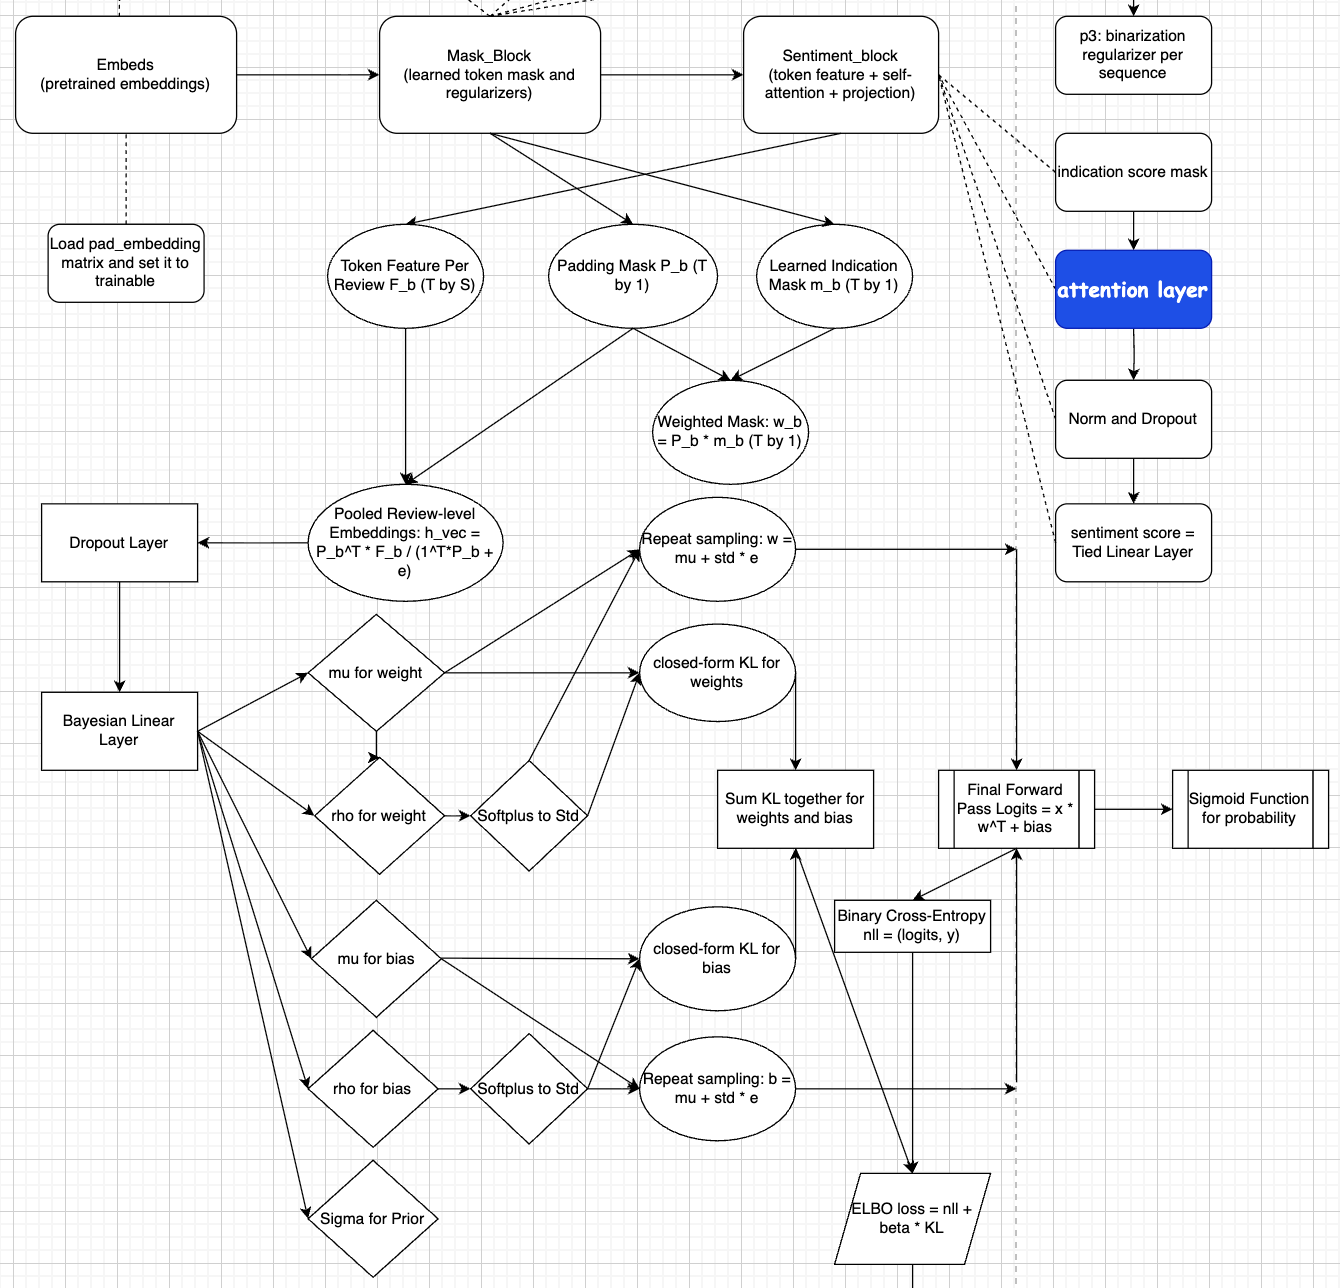
\includegraphics[width=1\linewidth]{Bayes.png}
    \caption{Bayesian Variational AMIC Architecture}
    \label{fig:Bayes}
\end{figure}

\section{word-level sentiment scores}
This section introduces the way we calculate the word-level sentiment scores from the above model. There are two ways to calculate the word-level sentiment scores. The first traditional approach involves obtaining word-level sentiment scores from the \textbf{Sentiment\_block} proposed by the original AMIC model. However, we don't use the word-level sentiment scores from \textbf{Sentiment\_block} as the last layer to calculate the logits with true labels. Thus, these sentiment scores are no longer accurate because they represent intermediate computation outcomes. As we discuss, the more accurate word-level sentiment scores are the final layer, which are the closest to the final logits. By the design of the backpropagation of the neural network, the word-level sentiment scores from a positive review would be pushed higher to close to positive labels. In contrast, word-level sentiment scores from a negative review would be pushed lower to close to negative labels. The second approach to calculating word-level sentiment scores involves passing word-level embeddings from \textbf{Sentiment\_block} to the Bayesian head's deterministic average weights, which yields the word-level logit contribution. This contribution is then averaged by word to obtain the final word-level sentiment scores. The formula would be: $$\text{word-level contribution}=\frac{\text{Bayesian head weights} \times \text{word-level embeddings}^T}{\text{number of valid tokens per review}}\times \text{padding\_mask}$$ After we have word-level sentiment contributions for each review, we calculate the average and standard deviation of these contribution by each word as the final word-level sentiment scores. The following table \ref{tab:PN} is a snapshot of the top 10 positive and negative words. From this table, we can tell every word falls into the right sentiment group. For example, the first word 'pumped' means excited in most tweets. 'nazi' in many tweets can either refer to historical Nazi Germany or its ideology to an extremist, thus it is the top one negative word. 
\begin{table}[htbp]
\centering
\caption{Top 10 Positive and Negative Words with Sentiment Scores in Twitter Dataset}
\label{tab:sentiment_words}
\begin{tabular}{l r l r}
\toprule
\multicolumn{2}{c}{\textbf{Positive Words}} & \multicolumn{2}{c}{\textbf{Negative Words}} \\
\cmidrule(lr){1-2} \cmidrule(lr){3-4}
Word & Score & Word & Score \\
\midrule
pumped      & 1.722 & nazi     & -1.659 \\
beauty    & 1.619 & racist     & -1.462 \\
happiness      & 1.586 & false        & -1.459 \\
perfect        & 1.585 & neo   & -1.409 \\
3d      & 1.578 & jail      & -1.388 \\
ashley      & 1.568 & charges    & -1.384 \\
enjoying        & 1.522 & fake     & -1.356 \\
cream        & 1.473 & nazis   & -1.280 \\
marley         & 1.456 & attacks     & -1.198 \\
beautiful      & 1.392 & charged     & -1.146 \\
\bottomrule
\end{tabular}
\label{tab:PN}
\end{table}
The table \ref{tab:PN} is an example of the Twitter dataset. We also experimented with the new model on four different datasets. We will discuss them in the next section. 

\section{Dataset}
We selected four benchmark datasets that have been extensively tested and utilized by researchers evaluating their new models. The first dataset is the wine review dataset proposed by Chenyu Yang in his dissertation thesis \cite{chenyu} in 2023. The second dataset is the Twitter dataset. Francesco Barbieri and other authors published a paper that includes heterogeneous tasks in Twitter, and all framed as multi-class tweet classification datasets in \cite{barbieri2020tweeteval}. Thus, we selected one of the sentiment analysis datasets from them as our benchmark dataset, as cited in \cite{rosenthal2017semeval}. The third dataset is the Amazon Polarity Classification Dataset published on Hugging Face by \cite{McAuley2013HiddenFA}, \cite{muennighoff2022mteb}, and \cite{enevoldsen2025mmtebmassivemultilingualtext}. The fourth dataset is the Large Movie Review Dataset proposed by \cite{maas-EtAl:2011:ACL-HLT2011} from IMDB.

\subsection{Wine Review Dataset}
Chenyu Yang \cite{chenyu} pulled the wine reviews from the website \hyperlink{https://www.winespectator.com/ratings}{wine spectator} in his dissertation for his original AMIC model. The following table \ref{tab:wine} is a snapshot of this data. The original data contains the following variables: wine name, vintage year, review year, rating score, price, wine reviewer, and clean description. The two variables we used are rating and Clean description. We cut off the threshold at 89 for rating scores. Reviews with ratings of 89 or higher are labeled as positive. The reviews with ratings less than or equal to 89 are labeled as negative. The column Clean\_desc is the text variable that we used to train the AMIC model. We split the data into training set, validation set and test set. We make every review equal length of 100 by either padding zeros at the beginning when the review is shorter than 100 or cutting off at 100th token of the review when it is longer than 100, and add one more digit as the 101th token at the end for each review which is the original review length for training. The training set shape is 127713 by 101. The validation set shape is 7095 by 101. The test set shape is 7096 by 101. The follow graph \ref{fig:wine_label} is the  whole dataset label distribution. As we can observe, the ratio of negative labels to positive labels is roughly equal to 2:1. This assures us that labels are still within the acceptable balance.  
\begin{table}[!ht]
\begin{threeparttable}
    \small
    \centering
   \begin{tabular}{|c|c|c|c|c|c|c|}
\hline name & vintage & review\_year & rating & price & reviewer & Clean\_desc \\
\hline 2 Up & 2004 & 2006 & 80 & 14 & hs & Smells great, but it's a bit tough and acidic ... \\
\hline 8 Golfo & NV & 2008 & 80 & 70 & tm & Grapey and chocolate flavors mingle in this fi... \\
\hline Acacia & 2011 & 2014 & 80 & 24 & jl & Smells of sautéed mushroom, soy and stale ging... \\
\hline Acacia & 2007 & 2009 & 80 & 26 & jl & Dry, earthy, herbal and dried currant and berr... \\
\hline Acacia & 2004 & 2006 & 80 & 50 & jl & Earthy and tilting toward barnyardy. Dry and a... \\
\hline
\end{tabular}
    \caption{Wine Review Dataset}
    \label{tab:wine}
\end{threeparttable}
\end{table}
\begin{figure}[!ht]
    \centering
    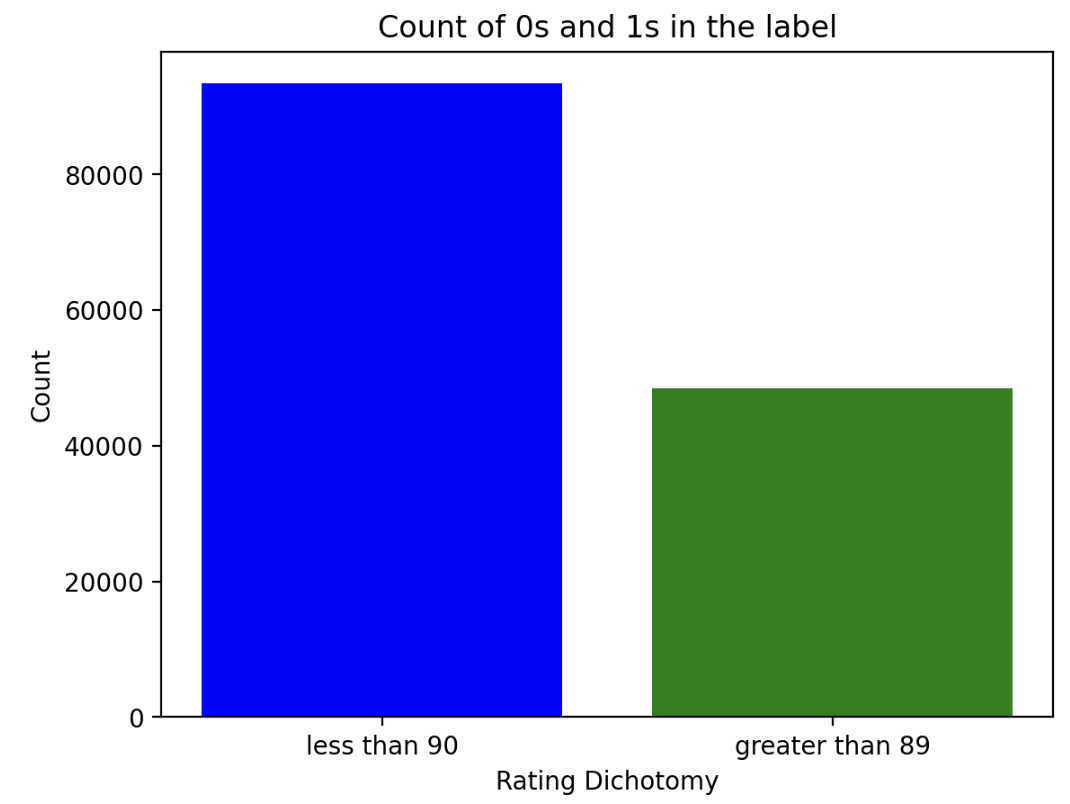
\includegraphics[width=0.5\linewidth]{wine label.png}
    \caption{The whole Wine Review label distribution}
    \label{fig:wine_label}
\end{figure}

\subsection{Twitter Dataset}
The Twitter Dataset we used is created by Rosenthal \cite{rosenthal2017semeval} in 2017 and they published their dataset and related paper on their public github website \hyperlink{https://github.com/cardiffnlp/tweeteval}{tweeteval}. The original Twitter dataset has three sentiment labels, positive, neutral and negative. However, to make our comparison consistently, we dropped all the neutral labels to keep it as a binary classification. The Twitter is imported by the python package \textit{datasets}. The following table \ref{tab:twitter} is the snapshot of this Twitter dataset. The Clean\_desc is the tweet texts, variable y is the sentiment labels and the split column is the indication of the split. Tweets are usually much shorter than wine reviews or other text descriptions, thus the average length of all tweets is 18.7. We selected the padding size to be 50 which can fully cover all the tweets in this dataset. The training set shape is 29178 by 51. The validation set shape is 1621 by 51. The test set shape is 1621 by 51. The following figure \ref{fig:twitter dist} is the twitter dataset label distribution. The ratio of positive labels to negative labels is roughly 2:1. It is still acceptable to train a binary classification task. The tweets are quite different from other regular reviews or text descriptions because it is shorter and contains some emojis, symbols and abbreviation, as a result, training Twitter dataset would be a more challenging task than other datasets. 
\begin{table}[!ht]
    \centering
    \begin{tabular}{|c|c|c|}
    \hline Clean\_desc & y & split \\
    \hline "QT @user In the original draft of the 7th boo... & 1 & train \\
    \hline @user Alciato: Bee will invest 150 million in ... & 1 & train \\
    \hline @user LIT MY MUM 'Kerry the louboutins I wonde... & 1 & train \\
    \hline "\"""" SOUL TRAIN $\backslash$ """" OCT 27 HALLOWEEN SPECIA... & 1 & train \\
    \hline So disappointed in wwe summerslam! I want to S... & 0 & train \\
    \hline
    \end{tabular}
    \caption{Twitter Dataset Snapshot}
    \label{tab:twitter}
\end{table}
\begin{figure}[!ht]
    \centering
    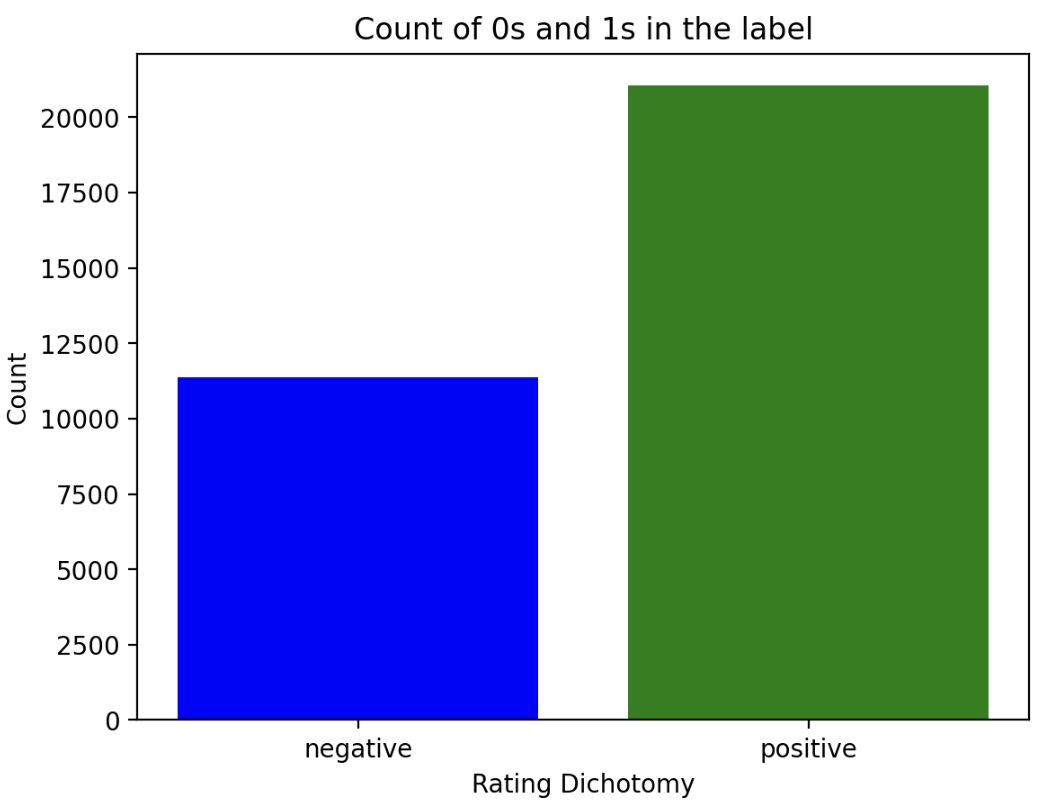
\includegraphics[width=0.5\linewidth]{twitter.png}
    \caption{Twitter Label distribution}
    \label{fig:twitter dist}
\end{figure}

\subsection{Amazon Review Dataset}
The third dataset we used is the Amazon Polarity Classification Dataset published on the Hugging Face website \hyperlink{https://huggingface.co/datasets/mteb/amazon_polarity}{Massive Text Embedding Benchmark}. The Amazon review is a very good example to evaluate the new language models. The original training set has 3,600,000 reviews and the original test set has 400,000 rows. The following table \ref{tab:amazon} is the snapshot of this Amazon review dataset. The column y indicates the sentiment labels. 1 means positive, while 0 means negative. Most Amazon reviews have less than 100 words per review, and the average length of reviews is 78. We selected the pad size of 224 to be unified length for each review that can cover every Amazon review. The final training set shape is 72000 by 225. The validation set shape is 4000 by 225. The test set shape is 4000 by 225. The following figure \ref{fig:amazon_label} is the Amazon dataset sentiment label distribution. As we can see, this dataset is selected to have the equal size of negative and positive labels, making the training more fair. 
\begin{table}[H]
    \centering
    \begin{tabular}{|c|p{16cm}|}
\hline y & Clean\_desc \\
\hline 1 & textbook Book shipped quickly and was in excellent condition as stated. Easy transaction would buy again  \\
\hline 1 & a great book for Historical romance lovers This is an engaging a count of life of Tess a girl who at a young age washed up on the shore of the Isle of May. With no memory of the life before then, she...\\
\hline 1 & YES!!! When I got this book, I wasn't expecting much, but man was I wrong! I loved this book! Now I may not usually be tied in by a man with long blond hair wearing a kilt, but the authors really mad...  \\
\hline 0 & Not the best in the series Tess Lindsay is content to be the sole occupant of a remote island but when Colin Macpherson washes ashore her life of solitude gets shaken up. Tess had always been told... \\
\hline 0 & ADDONICS PORTABLE CD DRIVE - I am disappointed in its performance I am disappointed in its performance. It seems underpowered and is constantly trying to read CDs, half the time... \\
\hline 0 & Too Uncomfortable and Too Big These pants were way too big (looked about 2 sizes larger), and they were incredibly stiff. They would have been very uncomfortable for my daughter to wear all day.\\
\hline 1 & Very authentic This is my first encounter with Yoruba and I have to say that CDs are really helping. However, the book is very short and not particular about certain aspects and details of grammar and... \\
\hline
\end{tabular}
    \caption{Amazon review dataset Snapshot}
    \label{tab:amazon}
\end{table}
\begin{figure}[H]
    \centering
    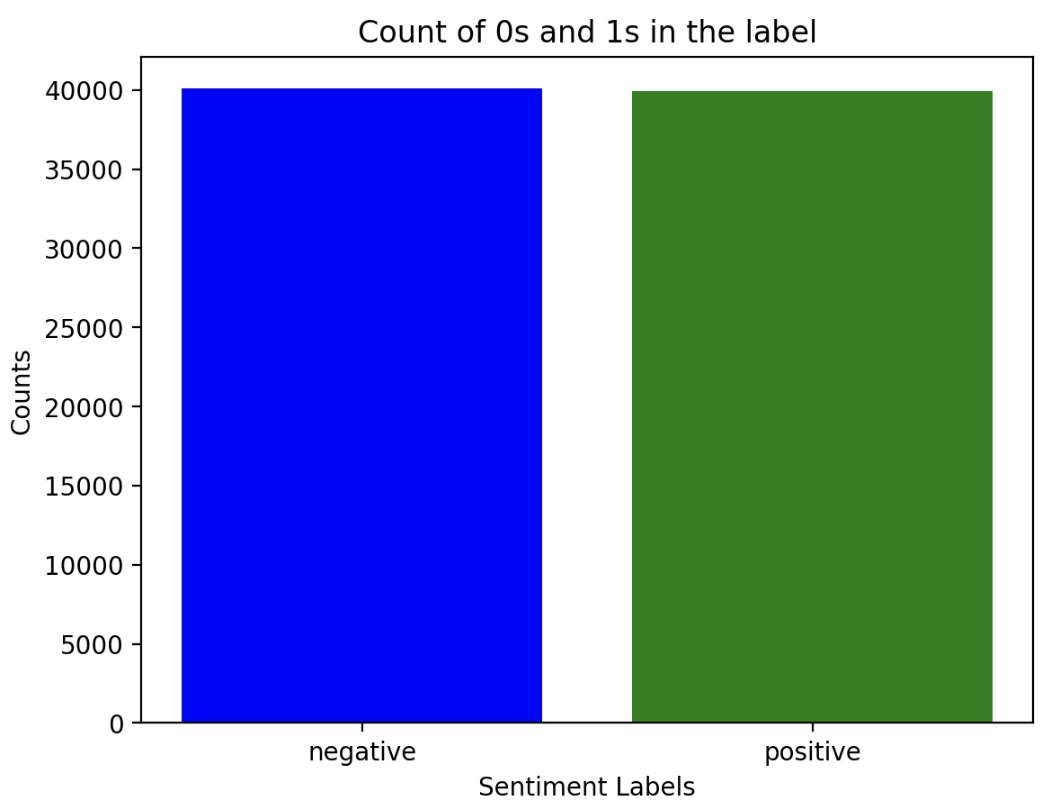
\includegraphics[width=0.5\linewidth]{amazon_labels.png}
    \caption{Amazon Label Distribution}
    \label{fig:amazon_label}
\end{figure}

\subsection{IMDB Dataset}
The last dataset we used is IMDB, Large Movie Review Dataset, published by Andrew L. Maas \cite{maas-etal-2011-learning} in 2011. This dataset contains 25,000 highly polar movie reviews for training, and 25,000 for testing. Andrew L. Maas \cite{maas-etal-2011-learning} in 2011 proposed a mix of unsupervised and supervised techniques to learn word vectors to capture rich sentiment content that is important for a varied of NLP task. They proposed this IMDB movie dataset to evaluate their new model and serve as a benchmark dataset for sentiment analysis. The average length for this movie review dataset is around 230. However, we selected 512 as our unified padding size for each review when 92\% percent of reviews in this dataset are less than 512 tokens. The following table \ref{tab:IMDB} is the snapshot of this dataset. As usual, 1 in column y means positive, and 0 in column y means negative. Our training set shape is 45000 by 513. The validation set shape is 2500 by 513. The test set shape is 2500 by 513. The following figure \ref{fig:imdb_label} shows this dataset has equal size of negative and positive labels to make the training exactly balance. 
\begin{table}[H]
    \centering
    \begin{tabular}{|l|c|}
\hline Clean\_desc & y \\
\hline I have always been a huge James Bond fanatic! ... & 1 \\
\hline I am a Christian and I say this movie had terr... & 0 \\
\hline Neatly sandwiched between THE STRANGER, a smal... & 1 \\
\hline Years ago I did follow a soap on TV. So I was ... & 1 \\
\hline Here's a gritty, get-the-bad guys revenge stor... & 1 \\
\hline
\end{tabular}
    \caption{IMDB Dataset Snapshot}
    \label{tab:IMDB}
\end{table}
\begin{figure}[H]
    \centering
    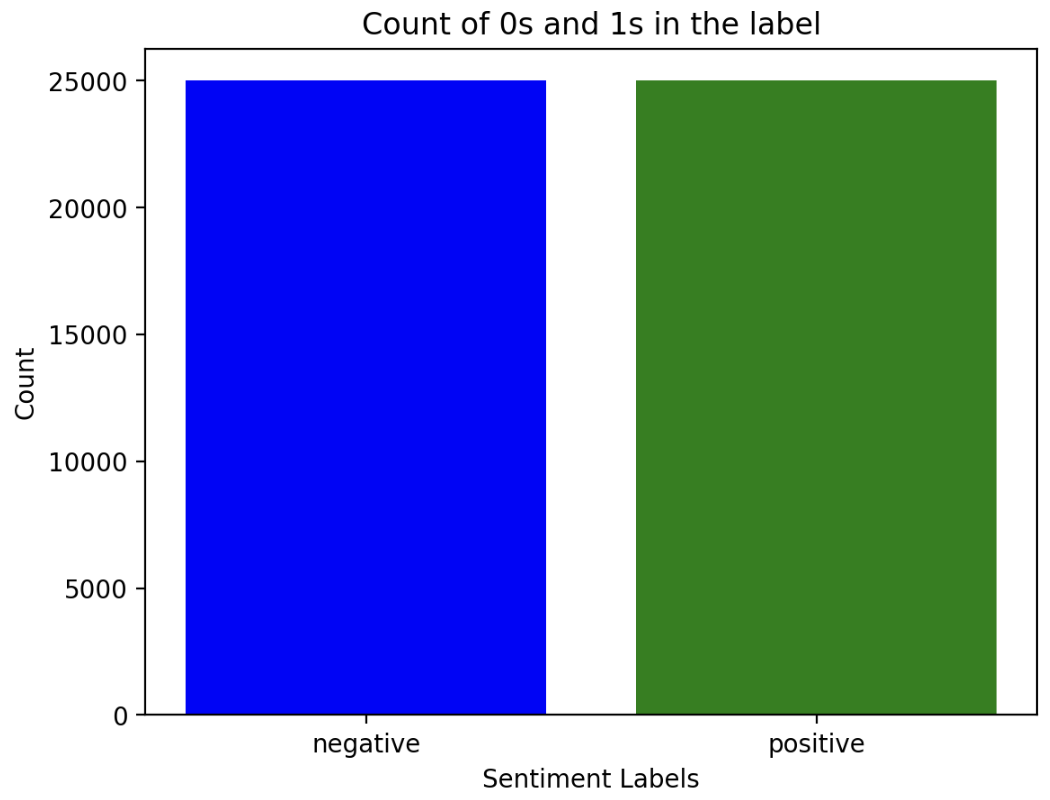
\includegraphics[width=0.5\linewidth]{IMDB labels.png}
    \caption{IMDB Label Distribution}
    \label{fig:imdb_label}
\end{figure}

\section{Training Results}
We trained the Bayesian Variational AMIC model on these four datasets. The following graphs are the training set accuracy and validation set accuracy changes against each epoch.   

\begin{figure}[htbp]
    \centering
    \begin{subfigure}{0.45\textwidth}
        \centering
        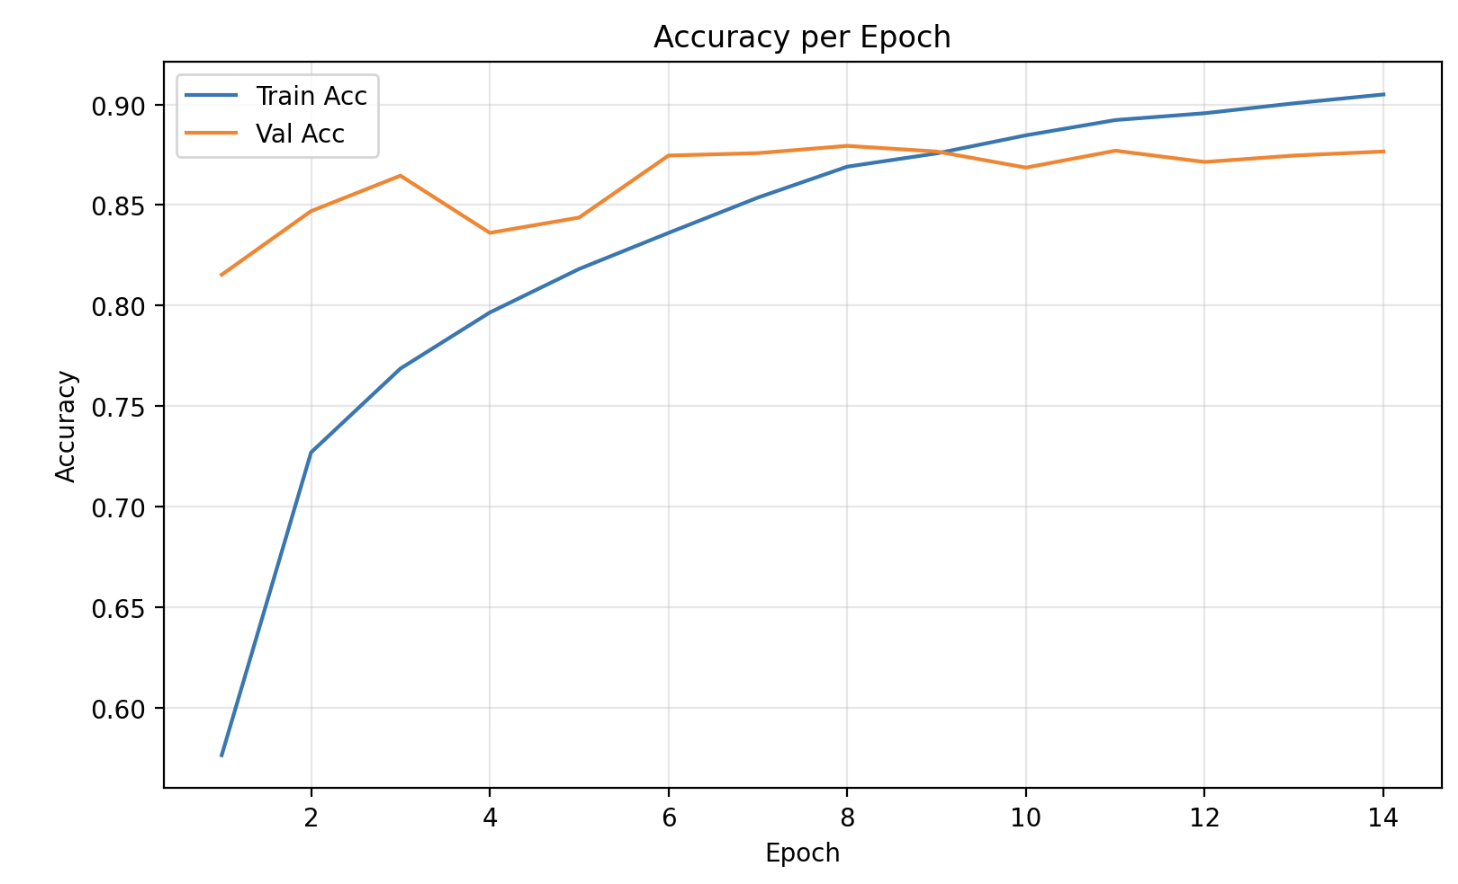
\includegraphics[width=\linewidth]{IMDB acc.png}
        \caption{IMDB Dataset Training and Validation Accuracy}
        \label{fig:imdb_acc}
    \end{subfigure}
    \hfill
    \begin{subfigure}{0.45\textwidth}
        \centering
        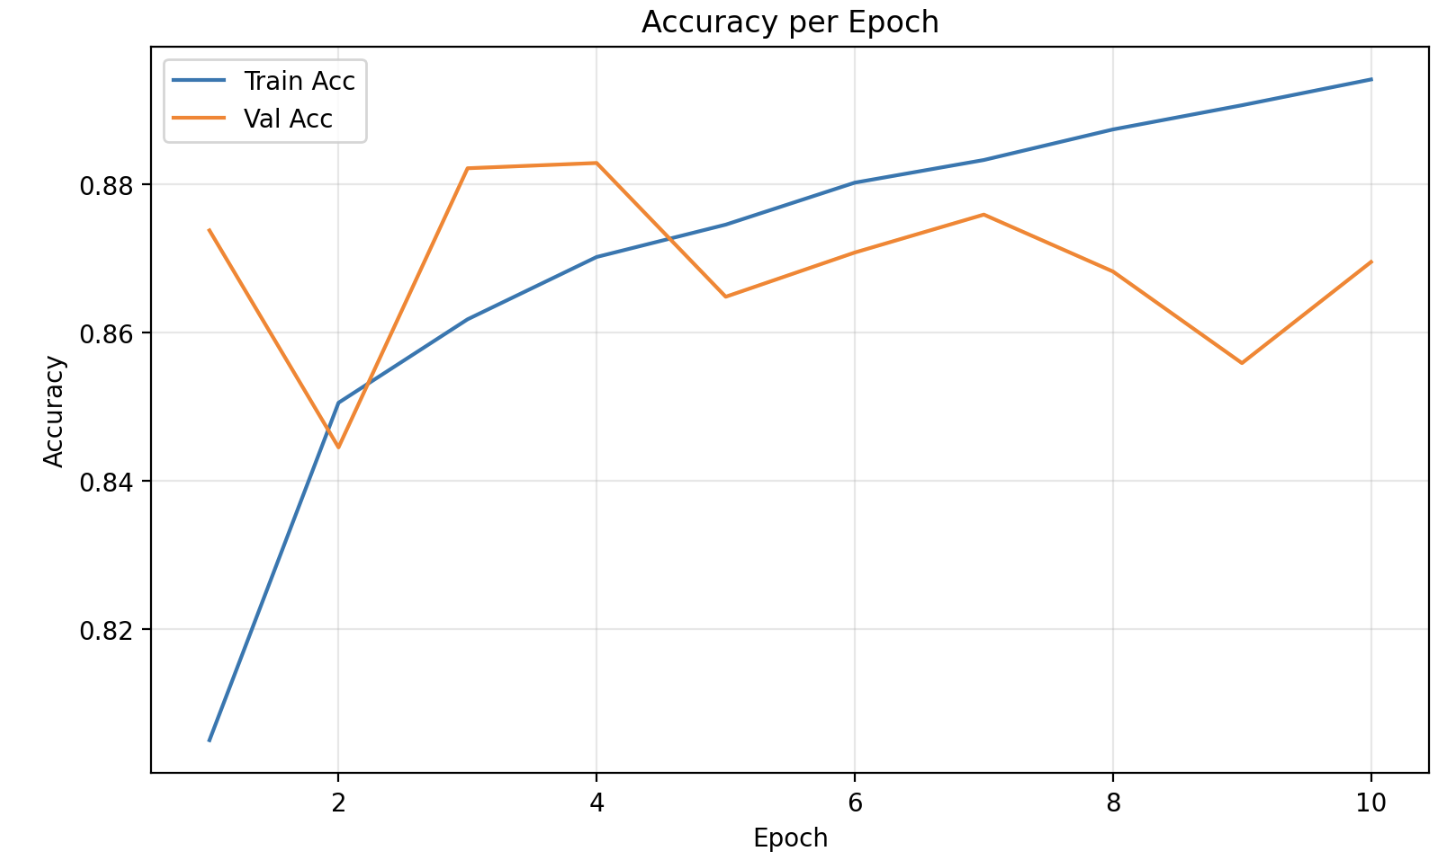
\includegraphics[width=\linewidth]{wine_acc.png}
        \caption{Wine Review Dataset Training and Validation Accuracy}
        \label{fig:wine_acc}
    \end{subfigure}
    
    \vspace{0.5cm} % Add some vertical space between rows
    
    \begin{subfigure}{0.45\textwidth}
        \centering
        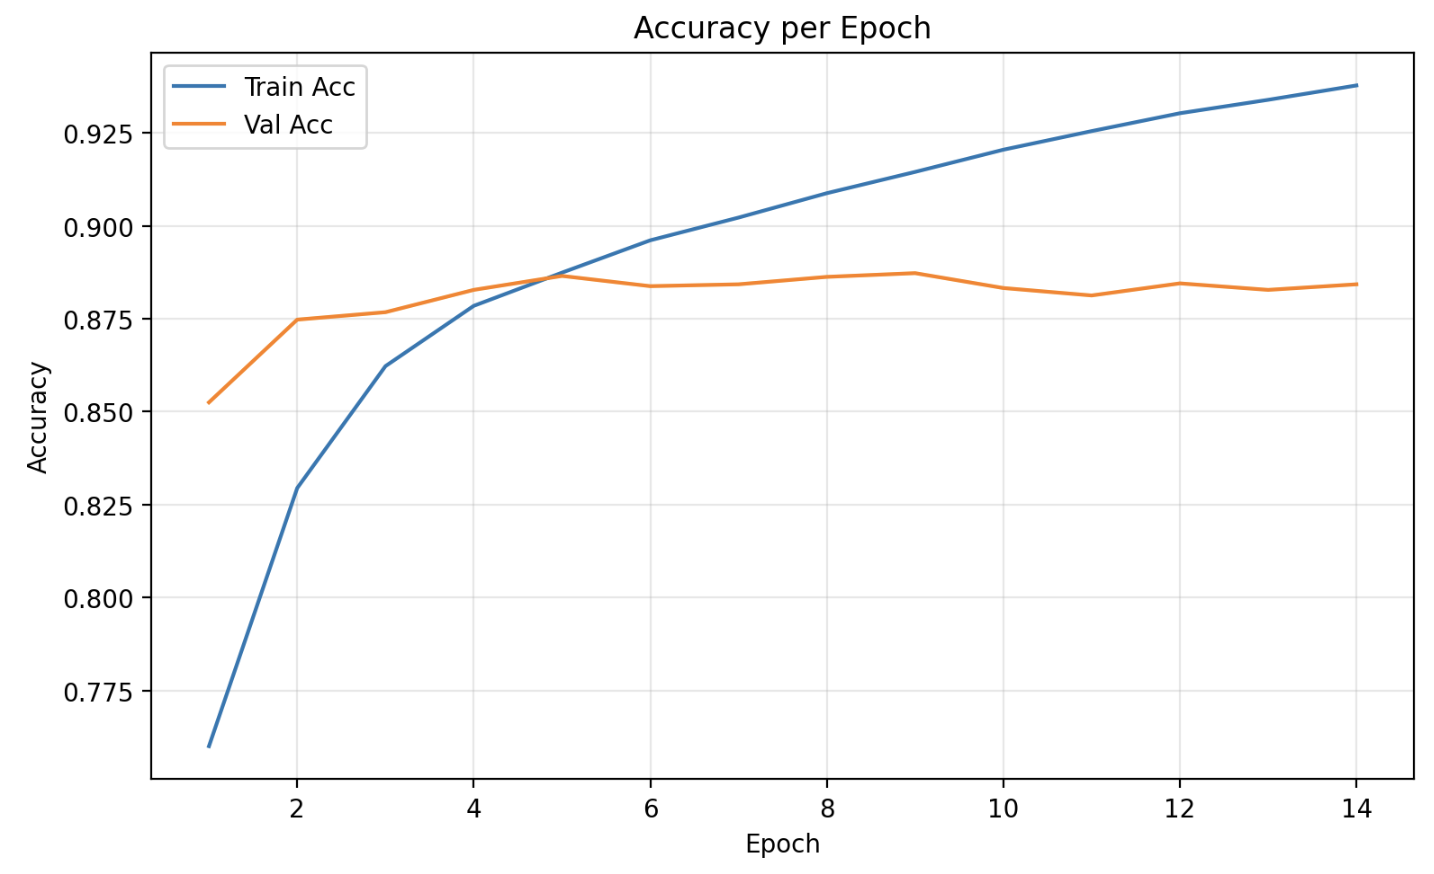
\includegraphics[width=\linewidth]{amazon_acc.png}
        \caption{Amazon Review Dataset Training and Validation Accuracy}
        \label{fig:amazon_acc}
    \end{subfigure}
    \hfill
    \begin{subfigure}{0.45\textwidth}
        \centering
        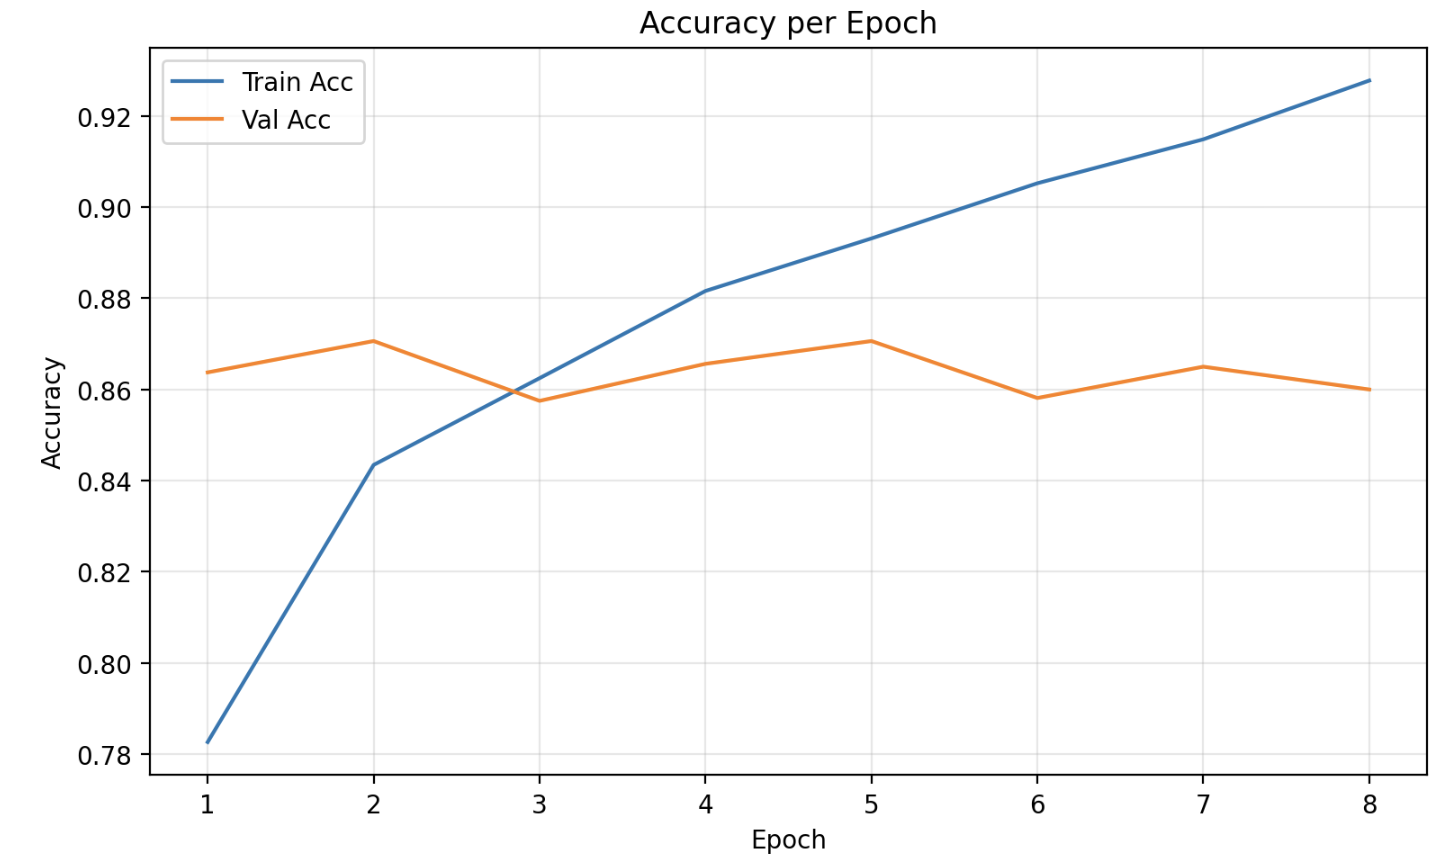
\includegraphics[width=\linewidth]{twitter_acc.png}
        \caption{Twitter Dataset Training and Validation Accuracy}
        \label{fig:twitter_acc}
    \end{subfigure}
    \caption{Training and validation accuracy for all datasets}
    \label{fig:all_accuracies}
\end{figure}
\printbibliography
\end{document}
